% LaTeX source for ``Think Stats:
% Probability and Statistics for Programmers''
% Copyright 2011  Allen B. Downey.

% License: Creative Commons Attribution-NonCommercial 3.0 Unported License.
% http://creativecommons.org/licenses/by-nc/3.0/
%

%\documentclass[10pt,b5paper]{book}
\documentclass[12pt]{book}
\usepackage[width=5.5in,height=8.5in,
  hmarginratio=3:2,vmarginratio=1:1]{geometry}

% for some of these packages, you might have to install
% texlive-latex-extra (in Ubuntu)

\usepackage[T1]{fontenc}
\usepackage{textcomp}
\usepackage{mathpazo}

%\usepackage{pslatex}

\usepackage{url}
\usepackage{fancyhdr}
\usepackage{graphicx}
\usepackage{subfig}
\usepackage{amsmath}
\usepackage{amsthm}
%\usepackage{amssymb}
\usepackage{makeidx}
\usepackage{setspace}
\usepackage{hevea}                           
\usepackage{upquote}


\title{Think Stats}
\author{Allen B. Downey}

\newcommand{\thetitle}{Think Stats: Probability and Statistics for Programmers}
\newcommand{\theversion}{1.5.9}

% these styles get translated in CSS for the HTML version
\newstyle{a:link}{color:black;}
\newstyle{p+p}{margin-top:1em;margin-bottom:1em}
\newstyle{img}{border:0px}

% change the arrows in the HTML version
\setlinkstext
  {\imgsrc[ALT="Previous"]{back.png}}
  {\imgsrc[ALT="Up"]{up.png}}
  {\imgsrc[ALT="Next"]{next.png}} 

\makeindex

\newif\ifplastex
\plastexfalse

\begin{document}

\frontmatter

\ifplastex
    \usepackage{localdef}
    \maketitle

\else

\input{latexonly}

\newtheoremstyle{exercise}% name of the style to be used
  {\topsep}% measure of space to leave above the theorem. E.g.: 3pt
  {\topsep}% measure of space to leave below the theorem. E.g.: 3pt
  {}% name of font to use in the body of the theorem
  {0pt}% measure of space to indent
  {\bfseries}% name of head font
  {}% punctuation between head and body
  { }% space after theorem head; " " = normal interword space
  {}% Manually specify head

\theoremstyle{exercise}
\newtheorem{exercise}{Exercise}[chapter]

\fi


\chapter{Preface}
\label{preface}

\section*{Why I wrote this book}

\newcommand{\tbl}[2]{#2\caption{#1}}

Figure~\ref{nsfg_hist} shows histograms of pregnancy lengths for
first babies and others.
\index{pregnancy length}
\index{length!pregnancy}

\begin{unnumlist}
\subparagraph{Accuracy}
\item \index{accuracy!defined} Accuracy expresses how close the result of a calculation
  or measurement comes to the ``true'' value. Low accuracy is due to
  systematic error.
\subparagraph{Precision} \index{precision!defined} 
\item Precision refers to the ``margin of error'' \index{margin of error} in the 
  calculation or the experiment. In experimental situations, precision
  tells us how far the results will stray when the experiment is 
  repeated several times. Low precision is due to random noise.
\end{unnumlist}


\begin{table}
\tbl{The first 30 job titles and their relative frequencies.\label{tbl:jobtitles}}{%
\begin{tabular}{lrrr}
\toprule
   & \textbf{Number of}
   & \textbf{Fraction of}
  & \textbf{Cumulative} \\
\textbf{Title} &  \textbf{customers} & \textbf{customers} & \textbf{fraction}\\
\colrule
Teacher \rule{0mm}{4mm}  & 66,470  &  0.34047   &   0.340 \\ 
Principal                & 22,958  &  0.11759   &   0.458 \\
Superintendent           & 12,521  &  0.06413   &   0.522 \\
\botrule
\end{tabular}}
\end{table}

{\em Think Stats: Probability and Statistics for Programmers} is a
textbook for a new kind of introductory prob-stat class.  
It emphasizes the use of statistics to explore large datasets.  It
takes a computational approach, which has several advantages:

\begin{itemize}

\item Students write programs as a way of developing and testing their
  understanding.  For example, they write functions to compute a least
  squares fit, residuals, and the coefficient of determination.
  Writing and testing this code requires them to understand the
  concepts and implicitly corrects misunderstandings.

\item Students run experiments to test statistical behavior.  For
  example, they explore the Central Limit Theorem (CLT) by generating
  samples from several distributions.  When they see that the sum of
  values from a Pareto distribution doesn't converge to normal, they
  remember the assumptions the CLT is based on.

\item Some ideas that are hard to grasp mathematically are easy to
  understand by simulation.  For example, we approximate p-values by
  running Monte Carlo simulations, which reinforces the meaning of the
  p-value.

\item Using discrete distributions and computation makes it possible
  to present topics like Bayesian estimation that are not usually
  covered in an introductory class.  For example, one exercise asks
  students to compute the posterior distribution for the ``German tank
  problem,'' which is difficult analytically but surprisingly easy
  computationally.

\item Because students work in a general-purpose programming language
  (Python), they are able to import data from almost any
  source.  They are not limited to data that has been cleaned and
  formatted for a particular statistics tool.

\end{itemize}

The book lends itself to a project-based approach.  In my class, students
work on a semester-long project that requires them to pose a statistical
question, find a dataset that can address it, and apply each of the
techniques they learn to their own data.

To demonstrate the kind of analysis I want students to do,
the book presents a case study that runs through all of the chapters.
It uses data from two sources:

\begin{itemize}

\item The National Survey of Family Growth (NSFG), conducted by the
  U.S. Centers for Disease Control and Prevention (CDC) to gather
  ``information on family life, marriage and divorce, pregnancy,
  infertility, use of contraception, and men's and women's health.''
  (See \url{http://cdc.gov/nchs/nsfg.htm}.)

\item The Behavioral Risk Factor Surveillance System (BRFSS),
  conducted by the National Center for Chronic Disease Prevention and
  Health Promotion to ``track health conditions and risk behaviors in
  the United States.''  (See \url{http://cdc.gov/BRFSS/}.)

\end{itemize}

Other examples use data from the IRS, the U.S. Census, and
the Boston Marathon.


\section*{How I wrote this book}

When people write a new textbook, they usually start by
reading a stack of old textbooks.  As a result, most books
contain the same material in pretty much the same order.  Often there
are phrases, and errors, that propagate from one book to the next;
Stephen Jay Gould pointed out an example in his essay, ``The Case of
the Creeping Fox Terrier\footnote{A breed of dog that is about half
  the size of a Hyracotherium (see
  \url{http://wikipedia.org/wiki/Hyracotherium}).}.''

I did not do that.  In fact, I used almost no printed material while I
was writing this book, for several reasons:

\begin{itemize}

\item My goal was to explore a new approach to this material, so I didn't
want much exposure to existing approaches.

\item Since I am making this book available under a free license, I wanted
to make sure that no part of it was encumbered by copyright restrictions.

\item Many readers of my books don't have access to libraries of
printed material, so I tried to make references to resources that are
freely available on the Internet.

\item Proponents of old media think that the exclusive
use of electronic resources is lazy and unreliable.  They might be right
about the first part, but I think they are wrong about the second, so
I wanted to test my theory.

% http://www.ala.org/ala/mgrps/rts/nmrt/news/footnotes/may2010/in_defense_of_wikipedia_bonnett.cfm

\end{itemize}

The resource I used more than any other is Wikipedia, the bugbear
of librarians everywhere.  In general, the articles I read on
statistical topics were very good (although I made a few small changes
along the way).  I include references to Wikipedia pages throughout
the book and I encourage you to follow those links; in many cases, the
Wikipedia page picks up where my description leaves off.  The
vocabulary and notation in this book are generally consistent with
Wikipedia, unless I had a good reason to deviate.

Other resources I found useful were Wolfram MathWorld and (of course)
Google.  I also used two books, David MacKay's {\em Information
  Theory, Inference, and Learning Algorithms}, which is the book that
got me hooked on Bayesian statistics, and Press et al.'s {\em
  Numerical Recipes in C}.  But both books are available online,
so I don't feel too bad.

Allen B. Downey \\*
Needham MA \\*

Allen B. Downey is a Professor of Computer Science at 
the Franklin W. Olin College of Engineering.



\section*{Contributor List}

If you have a suggestion or correction, please send email to 
{\tt downey@allendowney.com}.  If I make a change based on your
feedback, I will add you to the contributor list
(unless you ask to be omitted).
\index{contributors}

If you include at least part of the sentence the
error appears in, that makes it easy for me to search.  Page and
section numbers are fine, too, but not quite as easy to work with.
Thanks!

\small

\begin{itemize}

\item Lisa Downey and June Downey read an early draft and made many
corrections and suggestions.

\item Steven Zhang found several errors.

\item Andy Pethan and Molly Farison helped debug some of the solutions,
and Molly spotted several typos.

\item Andrew Heine found an error in my error function.

\item Dr. Nikolas Akerblom knows how big a Hyracotherium is.

\item Alex Morrow clarified one of the code examples.

\item Jonathan Street caught an error in the nick of time.

\item G\'{a}bor Lipt\'{a}k found a typo in the book and the relay race solution.

\item Many thanks to Kevin Smith and Tim Arnold for their work on
plasTeX, which I used to convert this book to DocBook.

\item George Caplan sent several suggestions for improving clarity.

\item Julian Ceipek found an error and a number of typos.

\item Stijn Debrouwere, Leo Marihart III, Jonathan Hammler, and Kent Johnson
found errors in the first print edition.

\item Dan Kearney found a typo.

\item Jeff Pickhardt found a broken link and a typo.

\item J\"{o}rg Beyer found typos in the book and made many corrections
in the docstrings of the accompanying code.

\item Tommie Gannert sent a patch file with a number of corrections.

% ENDCONTRIB

\end{itemize}

\normalsize

\clearemptydoublepage

% TABLE OF CONTENTS
\begin{latexonly}

\tableofcontents

\clearemptydoublepage

\end{latexonly}

% START THE BOOK
\mainmatter


\chapter{Statistical thinking for programmers}
\label{intro}

This book is about turning data into knowledge.  Data is cheap (at
least relatively); knowledge is harder to come by.

I will present three related pieces:

\begin{description}

\item[Probability] is the study of random events.  Most people have an
  intuitive understanding of degrees of probability, which is why you
  can use words like ``probably'' and ``unlikely'' without special
  training, but we will talk about how to make quantitative claims
  about those degrees.
\index{probability}

\item[Statistics] is the discipline of using data samples to support
  claims about populations.  Most statistical analysis is based on
  probability, which is why these pieces are usually presented
  together.
\index{statistics}

\item[Computation] is a tool that is well-suited to quantitative
  analysis, and computers are commonly used to process statistics.
  Also, computational experiments
  are useful for exploring concepts in probability and statistics.
\index{computation}

\end{description}

The thesis of this book is that if you know how to program, you can
use that skill to help you understand probability and statistics.
These topics are often presented from a mathematical perspective, and
that approach works well for some people.  But some important ideas
in this area are hard to work with mathematically and relatively
easy to approach computationally.

The rest of this chapter presents a case study motivated by a question
I heard when my wife and I were expecting our first child: do first
babies tend to arrive late?
\index{first babies}

\section{Do first babies arrive late?}

If you Google this question, you will find plenty of discussion.
Some people claim it's true, others say it's a myth, and some people
say it's the other way around: first babies come early.

In many of these discussions, people provide data to support their
claims.  I found many examples like these:

\begin{quote}

``My two friends that have given birth recently to their first babies,
BOTH went almost 2 weeks overdue before going into labour or being
induced.''

``My first one came 2 weeks late and now I think the second one is
going to come out two weeks early!!''

``I don't think that can be true because my sister was my mother's
first and she was early, as with many of my cousins.''

\end{quote}

Reports like these are called {\bf anecdotal evidence} because they
are based on data that is unpublished and usually personal.  In casual
conversation, there is nothing wrong with anecdotes, so I don't mean
to pick on the people I quoted.
\index{anecdotal evidence}

But we might want evidence that is more persuasive and
an answer that is more reliable.  By those standards, anecdotal
evidence usually fails, because:

\begin{description}

\item[Small number of observations:] If the gestation period is longer
  for first babies, the difference is probably small compared to the
  natural variation.  In that case, we might have to compare a large
  number of pregnancies to be sure that a difference exists.
\index{sample size}

\item[Selection bias:] People who join a discussion of this question
  might be interested because their first babies were late.  In that
  case the process of selecting data would bias the results.
\index{selection bias}
\index{bias!selection}

\item[Confirmation bias:] People who believe the claim might be more
  likely to contribute examples that confirm it.  People who doubt the
  claim are more likely to cite counterexamples.
\index{confirmation bias}
\index{bias!confirmation}

\item[Inaccuracy:] Anecdotes are often personal stories, and often
  misremembered, misrepresented, repeated
  inaccurately, etc.

\end{description}

So how can we do better?

\section{A statistical approach}

To address the limitations of anecdotes, we will use the tools
of statistics, which include:

\begin{description}

\item[Data collection:] We will use data from a large national survey
  that was designed explicitly with the goal of generating
  statistically valid inferences about the U.S. population.
\index{data collection}

\item[Descriptive statistics:] We will generate statistics that
  summarize the data concisely, and evaluate different ways to
  visualize data.
\index{descriptive statistics}

\item[Exploratory data analysis:] We will look for
  patterns, differences, and other features that address the questions
  we are interested in.  At the same time we will check for
  inconsistencies and identify limitations.
\index{exploratory data analysis}

\item[Hypothesis testing:] Where we see apparent effects, like a
  difference between two groups, we will evaluate whether the effect
  is real, or whether it might have happened by chance.
\index{hypothesis testing}

\item[Estimation:] We will use data from a sample to estimate
  characteristics of the general population.
\index{estimation}

\end{description}

By performing these steps with care to avoid pitfalls, we can
reach conclusions that are more justifiable and more likely to be
correct.


\section{The National Survey of Family Growth}
\label{nsfg}

Since 1973 the U.S. Centers for Disease Control and Prevention (CDC)
have conducted the National Survey of Family Growth (NSFG),
which is intended to gather ``information on family life, marriage and
divorce, pregnancy, infertility, use of contraception, and men's and
women's health. The survey results are used ... to plan health services and
health education programs, and to do statistical studies of families,
fertility, and health.''\footnote{See
  \url{http://cdc.gov/nchs/nsfg.htm}.}
\index{National Survey of Family Growth}
\index{NSFG}

We will use data collected by this survey to investigate whether first
babies tend to come late, and other questions.  In order to use this
data effectively, we have to understand the design of the study.

The NSFG is a {\bf cross-sectional} study, which means that it
captures a snapshot of a group at a point in time.  The most
common alternative is a {\bf longitudinal} study, which observes a
group repeatedly over a period of time.
\index{cross-sectional study}
\index{study!cross-sectional}
\index{longitudinal study}
\index{study!longitudinal}

The NSFG has been conducted seven times; each deployment is called
a {\bf cycle}.  We will be using data from Cycle 6, which was
conducted from January 2002 to March 2003.
\index{cycle}

The goal of the survey is to draw conclusions about a
{\bf population}; the target population of the NSFG is people in
the United States aged 15-44.
\index{population}

The people who participate in a survey are called {\bf respondents};
a group of respondents is called a {\bf cohort}.
In general, cross-sectional studies are meant to be {\bf
  representative}, which means that every member of the target
population has an equal chance of participating.  Of course that ideal
is hard to achieve in practice, but people who conduct surveys come as
close as they can.
\index{respondent}
\index{representative}

The NSFG is not representative; instead it is deliberately {\bf
  oversampled}.  The designers of the study recruited three
groups---Hispanics, African-Americans and teenagers---at rates higher
than their representation in the U.S. population.
The reason for oversampling is to make sure that the number of
respondents in each of these groups is large enough to draw valid
statistical inferences.
\index{oversampling}

Of course, the drawback of oversampling is that it is not as easy
to draw conclusions about the general population based on statistics
from the survey.  We will come back to this point later.

\begin{exercise}
Although the NSFG has been conducted seven times, it is not a
longitudinal study.  Read the Wikipedia pages
\url{http://wikipedia.org/wiki/Cross-sectional_study}
and
\url{http://wikipedia.org/wiki/Longitudinal_study}
to make sure you understand why not.
\end{exercise}

\begin{exercise}

In this exercise, you will download data from the NSFG; we will use
this data throughout the book.
\index{National Survey of Family Growth}
\index{NSFG}

\begin{enumerate}

\item Go to \url{http://thinkstats.com/nsfg.html}.  Read the terms of
use for this data and click ``I accept these terms'' (assuming that you do).

\item Download the files named {\tt 2002FemResp.dat.gz} and {\tt
  2002FemPreg.dat.gz}.  The first is the respondent file, which contains
  one line for each of the 7,643 female respondents.
  The second file contains one line for each pregnancy reported by a
  respondent.

\item Online documentation of the survey is at
  \url{http://www.icpsr.umich.edu/nsfg6}.
  Browse the sections in the left navigation bar to get a sense of
  what data are included.  You can also read the questionnaires
  at \url{http://cdc.gov/nchs/data/nsfg/nsfg_2002_questionnaires.htm}.

\item The web page for this book provides code to process the data
  files from the NSFG.  Download \url{http://thinkstats.com/survey.py}
  and run it in the same directory you put the data files in.  It
  should read the data files and print the number of lines in each:
\index{{\tt survey.py}}
%
\begin{verbatim}
Number of respondents 7643
Number of pregnancies 13593
\end{verbatim}

\item Browse the code to get a sense of what it does.  The next
section explains how it works.

\end{enumerate}

\end{exercise}

\section{Tables and records}

The poet-philosopher Steve Martin once said:
\index{Martin, Steve}
\index{oeuf}
\index{chapeau}
\index{French}
%
\begin{quote}
``Oeuf'' means egg, ``chapeau'' means hat.  It's like those French
  have a different word for everything.
\end{quote}
%
Like the French, database programmers speak a slightly
different language, and since we're working with a database we need
to learn some vocabulary.
\index{database}
\index{record (database)}
\index{field (database)}
\index{table (database)}

Each line in the respondents file contains information about one
respondent.  This information is called a {\bf record}.  The
variables that make up a record are called {\bf fields}.  A
collection of records is called a {\bf table}.
\index{{\tt survey.py}}

If you read {\tt survey.py} you will see class definitions for {\tt
  Record}, which is an object that represents a record, and {\tt
  Table}, which represents a table.

There are two subclasses of
{\tt Record}---{\tt Respondent} and {\tt Pregnancy}---which
contain records from the respondent and pregnancy tables.
For the time being, these classes are empty; in particular, there
is no init method to initialize their attributes.  Instead
we will use {\tt Table.MakeRecord} to convert a line of text into
a {\tt Record} object.
\index{init method}
\index{method!init}

There are also two subclasses of {\tt Table}: {\tt Respondents}
and {\tt Pregnancies}.  The init method in each class
specifies the default name of the data file and the type of
record to create.  Each {\tt Table} object has an attribute
named {\tt records}, which is a list of {\tt Record} objects.

For each {\tt Table}, the {\tt GetFields} method returns
a list of tuples that specify the fields from the record that
will be stored as attributes in each {\tt Record} object.  (You
might want to read that last sentence twice.)

For example, here is {\tt Pregnancies.GetFields}:
%
\begin{verbatim}
    def GetFields(self):
        return [
            ('caseid', 1, 12, int),
            ('prglength', 275, 276, int),
            ('outcome', 277, 277, int),
            ('birthord', 278, 279, int),
            ('finalwgt', 423, 440, float),
            ]
\end{verbatim}

The first tuple says that the field {\tt caseid} is in columns
1 through 12 and it's an integer.  Each tuple contains the following
information:

\begin{description}

\item[field:] The name of the attribute where the field
will be stored.  Most of the time I use the name from the
NSFG codebook, converted to all lower case.

\item[start:] The index of the starting column for this
field.
For example, the start index for {\tt caseid} is 1.
You can look up these indices in the NSFG codebook
at \url{http://nsfg.icpsr.umich.edu/cocoon/WebDocs/NSFG/public/index.htm}.

\item[end:] The index of the ending column for this
field; for example, the end index for {\tt caseid} is 12.
Unlike in Python, the end index is {\em inclusive}.

\item[conversion function:] A function that takes a string
and converts it to an appropriate type.  You can use built-in
functions, like {\tt int} and {\tt float}, or user-defined
functions.  If the conversion fails, the attribute gets the
string value {\tt 'NA'}.  If you don't want to convert a
field, you can provide an identity function or use {\tt str}.

\end{description}

For pregnancy records, we extract the following variables:

\begin{description}

\item[caseid] is the integer ID of the respondent.

\item[prglength] is the integer duration of the pregnancy in weeks.

\item[outcome] is an integer code for the outcome of the pregnancy.
The code 1 indicates a live birth.

\item[birthord] is the integer birth order of each live birth;
for example, the code for a first child is 1. 
For outcomes other than live birth, this field is blank.

\item[finalwgt] is the statistical weight associated with the respondent.
It is a floating-point value that indicates the number of people in
the U.S. population this respondent represents.  Members of oversampled
groups have lower weights.\index{weight!sample}

\end{description}

If you read the casebook carefully, you will see that most of these
variables are {\bf recodes}, which means that they are not part
of the {\bf raw data} collected by the survey, but they are
calculated using the raw data.
\index{recode}
\index{raw data}

For example, {\tt prglength} for live births is equal to the raw
variable {\tt wksgest} (weeks of gestation) if it is available;
otherwise it is estimated using {\tt mosgest * 4.33} (months of
gestation times the average number of weeks in a month).

Recodes are often based on logic that checks the consistency and
accuracy of the data.  In general it is a good idea to use recodes
unless there is a compelling reason to process the raw data
yourself.

You might also notice that {\tt Pregnancies} has a method called
{\tt Recode} that does some additional checking and recoding.

\begin{exercise}
In this exercise you will write a program to explore the data
in the Pregnancies table.

\begin{enumerate}

\item In the directory where you put {\tt survey.py} and the
data files, create a file named \verb"first.py" and
type or paste in the following code:
\index{{\tt survey.py}}
\index{{\tt first.py}}
%
\begin{verbatim}
import survey
table = survey.Pregnancies()
table.ReadRecords()
print 'Number of pregnancies', len(table.records)
\end{verbatim}

The result should be 13593 pregnancies.

\item Write a loop that iterates \verb"table" and counts
the number of live births.  Find the documentation of {\tt outcome}
and confirm that your result is consistent with the summary
in the documentation.

\item Modify the loop to partition the live birth records into
two groups, one for first babies and one for the others.  Again,
read the documentation of {\tt birthord} to see if your results
are consistent.

When you are working with a new dataset, these kinds of checks
are useful for finding errors and inconsistencies in the data,
detecting bugs in your program, and checking your understanding
of the way the fields are encoded.

\item Compute the average pregnancy length (in weeks) for first
babies and others.  Is there a difference between the groups?  How
big is it?
\index{pregnancy length}
\index{length!pregnancy}

\end{enumerate}

You can download a solution to this exercise from
\url{http://thinkstats.com/first.py}.\index{{\tt first.py}}

\end{exercise}


\section{Significance}

In the previous exercise, you compared the gestation period for first
babies and others; if things worked out, you found that first
babies are born about 13 hours later, on average.
\index{apparent effect}

A difference like that is called an {\bf apparent effect}; that is,
there might be something going on, but we are not yet sure.  There are
several questions we still want to ask:

\begin{itemize}

\item If the two groups have different means, what about other {\bf
  summary statistics}, like median and variance?  Can we be more
  precise about how the groups differ?
\index{summary statistic}

\item Is it possible that the difference we saw could occur by chance,
  even if the groups we compared were actually the same?  If so,
  we would conclude that the effect was not {\bf statistically
    significant}.
\index{statistically significant}
\index{significance}


\item Is it possible that the apparent effect is due to selection bias or
  some other error in the experimental setup?  If so, then we might
  conclude that the effect is an {\bf artifact}; that is, something we
  created (by accident) rather than found. 
\index{artifact}

\end{itemize}

Answering these questions will take most of the rest of this book.


\begin{exercise}
The best way to learn about statistics is to work on a project you are
interested in.  Is there a question like, ``Do first babies arrive
late,'' that you would like to investigate?

Think about questions you find personally interesting, or items of
conventional wisdom, or controversial topics, or questions that have
political consequences, and see if you can formulate a question that
lends itself to statistical inquiry.

Look for data to help you address the question.  Governments are good
sources because data from public research is often freely
available\footnote{On the day I wrote this paragraph, a court in the
  UK ruled that the Freedom of Information Act applies to scientific
  research data.}.

Another way to find data is Wolfram Alpha, which is a curated
collection of good-quality datasets at \url{http://wolframalpha.com}.
Results from Wolfram Alpha are subject to copyright
restrictions; you might want to check the terms before you commit
yourself.

Google and other search engines can also help you find data, but it
can be harder to evaluate the quality of resources on the web.

If it seems like someone has answered your question, look closely to
see whether the answer is justified.  There might be flaws in the data
or the analysis that make the conclusion unreliable.  In that case you
could perform a different analysis of the same data, or look for a
better source of data.

If you find a published paper that addresses your question, you
should be able to get the raw data.  Many authors make their data
available on the web, but for sensitive data you might have to
write to the authors, provide information about how you plan to use
the data, or agree to certain terms of use.  Be persistent!

\end{exercise}


\section{Glossary}

\begin{description}

\item[anecdotal evidence:] Evidence, often personal, that is collected
  casually rather than by a well-designed study.
\index{anecdotal evidence}

\item[population:] A group we are interested in studying, often a
  group of people, but the term is also used for animals, vegetables
  and minerals\footnote{If you don't recognize this phrase, see
    \url{http://wikipedia.org/wiki/Twenty_Questions}.}.
\index{population}

\item[cross-sectional study:] A study that collects data about a
population at a particular point in time.
\index{cross-sectional study}
\index{study!cross-sectional}

\item[longitudinal study:] A study that follows a population over
time, collecting data from the same group repeatedly.
\index{longitudinal study}
\index{study!longitudinal}

\item[respondent:] A person who responds to a survey.
\index{respondent}

\item[cohort:] A group of respondents
\index{cohort}

\item[sample:] The subset of a population used to collect data.
\index{sample}

\item[representative:] A sample is representative if every member
of the population has the same chance of being in the sample.
\index{representative}

\item[oversampling:] The technique of increasing the representation
of a sub-population in order to avoid errors due to small sample
sizes.
\index{oversampling}

\item[record:] In a database, a collection of information about
a single person or other object of study.
\index{record}

\item[field:] In a database, one of the named variables that makes
up a record.
\index{field}

\item[table:] In a database, a collection of records.
\index{table}

\item[raw data:] Values collected and recorded with little or no
checking, calculation or interpretation.
\index{raw data}

\item[recode:] A value that is generated by calculation and other
logic applied to raw data.
\index{recode}

\item[summary statistic:] The result of a computation that reduces
a dataset to a single number (or at least a smaller set of numbers)
that captures some characteristic of the data.
\index{summary statistic}

\item[apparent effect:] A measurement or summary statistic that
suggests that something interesting is happening.
\index{apparent effect}

\item[statistically significant:] An apparent effect is statistically
  significant if it is unlikely to occur by chance.
\index{statistically significant}

\item[artifact:] An apparent effect that is caused by bias,
  measurement error, or some other kind of error.
\index{artifact}

\end{description}



\chapter{Descriptive statistics}
\label{descriptive}

\section{Means and averages}
\label{mean}

In the previous chapter, I mentioned three summary statistics---mean,
variance and median---without explaining what they are.  So before
we go any farther, let's take care of that.
\index{mean}
\index{average}
\index{descriptive statistics}
\index{summary statistics}

If you have a sample of $n$ values, $x_i$, the mean, $\mu$, is
the sum of the values divided by the number of values; in other words
%
\[ \mu = \frac{1}{n} \sum_i x_i \]
%
The words ``mean'' and ``average'' are sometimes used interchangeably,
but I will maintain this distinction:

\begin{itemize}

\item The ``mean'' of a sample is the summary statistic computed with
  the previous formula.

\item An ``average'' is one of many summary statistics you might
  choose to describe the typical value or the
  {\bf central tendency} of a sample.
\index{central tendency}

\end{itemize}

Sometimes the mean is a good description of a set of values.  For
example, apples are all pretty much the same size (at least the ones
sold in supermarkets).  So if I buy 6 apples and the total weight is 3
pounds, it would be a reasonable summary to say they are about a half
pound each.
\index{weight!pumpkin}

But pumpkins are more diverse.  Suppose I grow several varieties in my
garden, and one day I harvest three decorative pumpkins that are 1
pound each, two pie pumpkins that are 3 pounds each, and one Atlantic
Giant\textregistered~pumpkin that weighs 591 pounds.  The mean of
this sample is 100 pounds, but if I told you ``The average pumpkin
in my garden is 100 pounds,'' that would be wrong, or at least
misleading.
\index{pumpkin}

In this example, there is no meaningful average because
there is no typical pumpkin.

\section{Variance}
\index{variance}

If there is no single number that summarizes pumpkin weights,
we can do a little better with two numbers: mean and {\bf variance}.

In the same way that the mean is intended to describe the central
tendency, variance is intended to describe the {\bf spread}.
The variance of a set of values is
%
\[ \sigma^2 = \frac{1}{n} \sum_i (x_i - \mu)^2 \]
%
The term $x_i - \mu$ is called the ``deviation from the mean,'' so
variance is the mean squared deviation, which is why it is denoted
$\sigma^2$.  The square root of variance, $\sigma$, is called the {\bf
  standard deviation}.
\index{deviation}
\index{standard deviation}

By itself, variance is hard to interpret.  One problem is that the
units are strange; in this case the measurements are in pounds, so the
variance is in pounds squared.  Standard deviation is more meaningful;
in this case the units are pounds.

\begin{exercise}
For the exercises in this chapter you should download
\url{http://thinkstats.com/thinkstats.py}, which contains general-purpose
functions we will use throughout the book.  You can read documentation
of these functions in \url{http://thinkstats.com/thinkstats.html}.
\index{{\tt thinkstats.py}}

Write a function called
{\tt Pumpkin} that uses functions from {\tt thinkstats.py} to compute
the mean, variance and standard deviation of the pumpkins weights in
the previous section.
\end{exercise}

\begin{exercise}
Reusing code from {\tt survey.py} and {\tt first.py}, compute the
standard deviation of gestation time for first babies and others.
Does it look like the spread is the same for the two groups?
\index{{\tt survey.py}}
\index{{\tt first.py}}

How big is the difference in the means compared to these standard
deviations?  What does this comparison suggest about the statistical
significance of the difference?
\end{exercise}

If you have prior experience, you might have seen a formula for
variance with $n-1$ in the denominator, rather than $n$.  This
statistic is called the ``sample variance,'' and it is used to
estimate the variance in a population using a sample.  We will come
back to this in Chapter X.  \index{sample variance}

\section{Distributions}
\label{distributions}
\index{distribution}

Summary statistics are concise, but dangerous, because they obscure
the data.  An alternative is to look at the {\bf distribution} of the
data, which describes how often each value appears.

The most common representation of a distribution is a {\bf histogram},
which is a graph that shows the frequency or probability
of each value.\index{histogram}

In this context, {\bf frequency} means the number of times a value
appears in a dataset---it has nothing to do with the pitch of a sound
or tuning of a radio signal.  A {\bf probability} is a frequency expressed
as a fraction of the sample size, $n$.
\index{frequency}
\index{probability}
\index{dictionary}

In Python, an efficient way to compute frequencies is with a dictionary.
Given a sequence of values, {\tt t}:
%
\begin{verbatim}
hist = {}
for x in t:
    hist[x] = hist.get(x, 0) + 1
\end{verbatim}

The result is a dictionary that maps from values to frequencies.
To get from frequencies to probabilities, we divide through by $n$,
which is called {\bf normalization}:\index{normalization}
%
\begin{verbatim}
n = float(len(t))
pmf = {}
for x, freq in hist.items():
    pmf[x] = freq / n
\end{verbatim}

The normalized histogram is called a {\bf PMF}, which stands for
``probability mass function''; that is, it's a function that maps from
values to probabilities (I'll explain ``mass'' in
Section X.X).
\index{PMF}
\index{probability mass function}

It might be confusing to call a Python dictionary a function.  In
mathematics, a function is a map from one set of values to
another.  In Python, we {\em usually} represent mathematical functions
with function objects, but in this case we are using a dictionary
(dictionaries are also called ``maps,'' if that helps).\index{map}


\section{Representing histograms}
\index{histogram}
\index{Hist object}
\index{{\tt pmf.py}@{\tt Pmf.py}}

I wrote a Python module called {\tt Pmf.py} that contains class
definitions for Hist objects, which represent histograms, and Pmf
objects, which represent PMFs.  You can read the documentation at {\tt
  thinkstats.com/Pmf.html} and download the code from {\tt
  thinkstats.com/Pmf.py}.

The function {\tt MakeHistFromList} takes a list of values and
returns a new Hist object.  You can test it in Python's interactive
mode:
%
\begin{verbatim}
>>> import Pmf
>>> hist = Pmf.MakeHistFromList([1, 2, 2, 3, 5])
>>> print hist
<Pmf.Hist object at 0xb76cf68c>
\end{verbatim}

{\tt Pmf.Hist} means that this object is a member of the Hist class,
which is defined in the Pmf module.  In general, I use upper case
letters for the names of classes and functions, and lower case letters
for variables.

Hist objects provide methods to look up values and their
probabilities.  {\tt Freq} takes a value and returns its frequency:
%
\begin{verbatim}
>>> hist.Freq(2)
2
\end{verbatim}

If you look up a value that has never appeared, the frequency is 0.
%
\begin{verbatim}
>>> hist.Freq(4)
0
\end{verbatim}

{\tt Values} returns an unsorted list of the values in the Hist:
%
\begin{verbatim}
>>> hist.Values()
[1, 5, 3, 2]
\end{verbatim}

To loop through the values in order, you can use the built-in function
{\tt sorted}:
%
\begin{verbatim}
for val in sorted(hist.Values()):
    print val, hist.Freq(val)
\end{verbatim}

If you are planning to look up all of the frequencies, it is more
efficient to use {\tt Items}, which returns an unsorted list of
value-frequency pairs:
%
\begin{verbatim}
for val, freq in hist.Items():
     print val, freq
\end{verbatim}

\begin{exercise}
The mode of a distribution is the most frequent value (see
\url{http://wikipedia.org/wiki/Mode_(statistics)}).  Write a function called
    {\tt Mode} that takes a Hist object and returns the most frequent
    value.\index{mode}

As a more challenging version, write a function called {\tt AllModes}
that takes a Hist object and returns a list of value-frequency
pairs in descending order of frequency.  Hint: the {\tt operator}
module provides a function called {\tt itemgetter} which you can
pass as a key to {\tt sorted}.

\end{exercise}


\section{Plotting histograms}
\index{plotting}
\index{{\tt pyplot}}

There are a number of Python packages for making figures and graphs.
The one I will demonstrate is {\tt pyplot}, which is part of
the {\tt matplotlib} package at \url{http://matplotlib.sourceforge.net}.

This package is included in many Python installations.  To see whether
you have it, launch the Python interpreter and run:
%
\begin{verbatim}
import matplotlib.pyplot as pyplot
pyplot.pie([1,2,3])
pyplot.show()
\end{verbatim}

If you have {\tt matplotlib} you should see a simple pie chart;
otherwise you will have to install it.
\index{matplotlib}
\index{bar plot}
\index{plot!bar}

Histograms and PMFs are most often plotted as bar charts.  The
{\tt pyplot} function to draw a bar chart is {\tt bar}.  Hist
objects provide a method called {\tt Render} that returns a sorted
list of values and a list of the corresponding frequencies, which
is the format {\tt bar} expects:
%
\begin{verbatim}
>>> vals, freqs = hist.Render()
>>> rectangles = pyplot.bar(vals, freqs)
>>> pyplot.show()
\end{verbatim}

I wrote a module called {\tt myplot.py} that provides functions
for plotting histograms, PMFs and other objects we will see soon.
You can read the documentation at {\tt
  thinkstats.com/myplot.html} and download the code from {\tt
  thinkstats.com/myplot.py}.  Or you can use
{\tt pyplot} directly, if you prefer.  Either way, you can find
the documentation for {\tt pyplot} on the web.
\index{{\tt myplot.py}}

Figure~\ref{nsfg_hist} shows histograms of pregnancy lengths for
first babies and others.
\index{pregnancy length}
\index{length!pregnancy}

\begin{figure}
% descriptive.py
\centerline{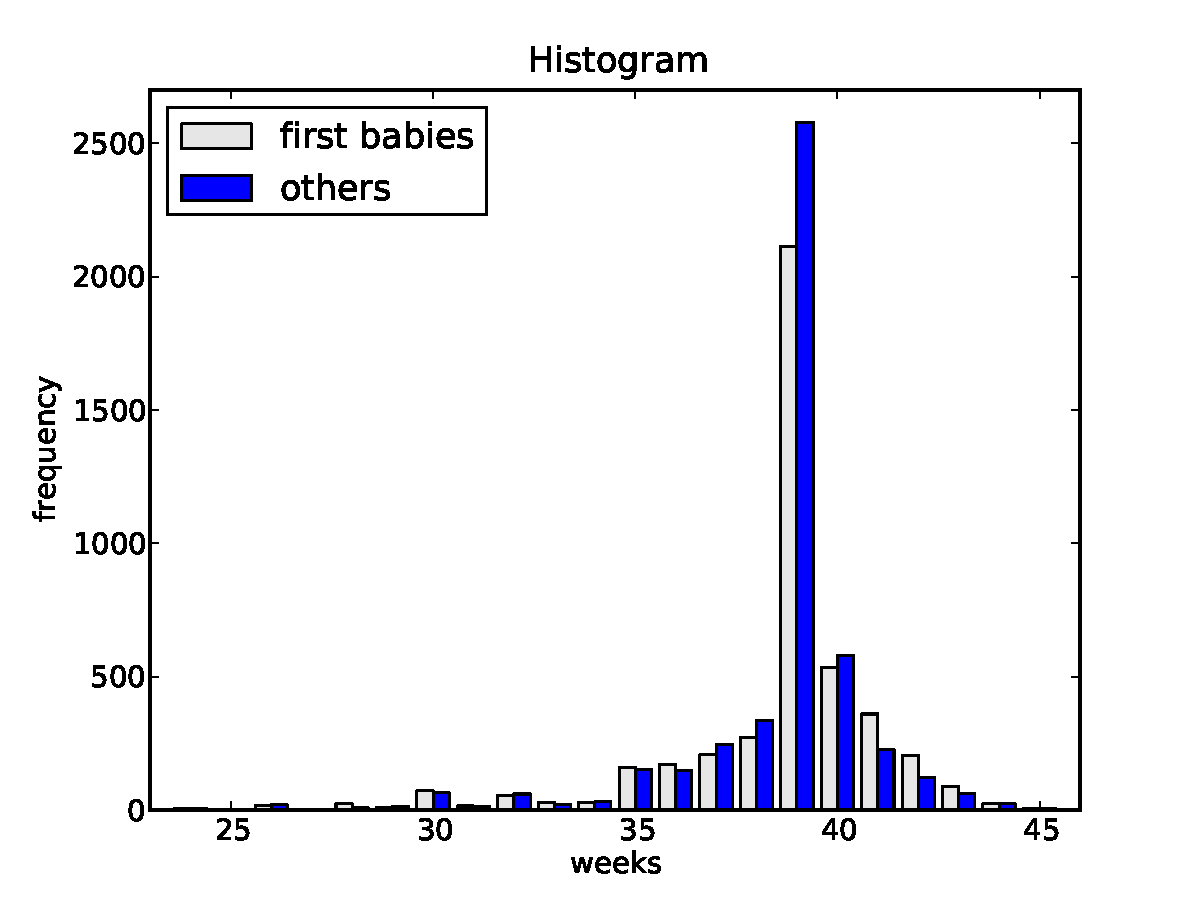
\includegraphics[height=2.5in]{figs/nsfg_hist.pdf}}
\caption{Histogram of pregnancy lengths.}
\label{nsfg_hist}
\end{figure}

Histograms are useful because they make the following features immediately
apparent:

\begin{description}

\item[Mode:] The most common value in a distribution is called the
  {\bf mode}.  In Figure~\ref{nsfg_hist} there is a clear mode at 39
  weeks.  In this case, the mode is the summary statistic that does
  the best job of describing the typical value.
\index{mode}

\item[Shape:] Around the mode, the distribution is asymmetric; it
  drops off quickly to the right and more slowly to the left.  From a
  medical point of view, this makes sense.  Babies are often born
  early, but seldom later than 42 weeks.  Also, the right side of the
  distribution is truncated because doctors often intervene after 42
  weeks.
\index{shape}

\item[Outliers:] Values far from the mode are called {\bf outliers}.
  Some of these are just unusual cases, like babies born at 30 weeks.
  But many of them are probably due to errors, either in the reporting
  or recording of data.
\index{outlier}

\end{description}

Although histograms make some features apparent, they are usually not
useful for comparing two distributions.  In this example, there are
fewer ``first babies'' than ``others,'' so some of the apparent
differences in the histograms are due to sample sizes.  We can
address this problem using PMFs.


\section{Representing PMFs}
\index{Pmf object}
\index{{\tt pmf.py}@{\tt Pmf.py}}

{\tt Pmf.py} provides a class called {\tt Pmf} that represents PMFs.
The notation can be confusing, but here it is: {\tt Pmf} is the
name of the module and also the class, so the full name of the class
is {\tt Pmf.Pmf}.  I often use {\tt pmf} as a variable name.
Finally, in the text, I use PMF to refer to the general concept
of a probability mass function, independent of my implementation.

To create a Pmf object, use {\tt MakePmfFromList}, which takes a list
of values:
%
\begin{verbatim}
>>> import Pmf
>>> pmf = Pmf.MakePmfFromList([1, 2, 2, 3, 5])
>>> print pmf
<Pmf.Pmf object at 0xb76cf68c>
\end{verbatim}

Pmf and Hist objects are similar in many ways.  The methods {\tt
  Values} and {\tt Items} work the same way for both types.  The
biggest difference is that a Hist maps from values to integer
counters; a Pmf maps from values to floating-point probabilities.

To look up the probability associated with a value, use {\tt Prob}:
%
\begin{verbatim}
>>> pmf.Prob(2)
0.4
\end{verbatim}

You can modify an existing Pmf by incrementing the probability
associated with a value:
%
\begin{verbatim}
>>> pmf.Incr(2, 0.2)
>>> pmf.Prob(2)
0.6
\end{verbatim}

Or you can multiply a probability by a factor:
%
\begin{verbatim}
>>> pmf.Mult(2, 0.5)
>>> pmf.Prob(2)
0.3
\end{verbatim}

If you modify a Pmf, the result may not be normalized; that is, the
probabilities may no longer add up to 1.  To check, you can call {\tt
  Total}, which returns the sum of the probabilities:
%
\begin{verbatim}
>>> pmf.Total()
0.9
\end{verbatim}

To renormalize, call {\tt Normalize}:
%
\begin{verbatim}
>>> pmf.Normalize()
>>> pmf.Total()
1.0
\end{verbatim}

Pmf objects provide a {\tt Copy} method so you can make and
and modify a copy without affecting the original.

\begin{exercise}
According to Wikipedia, ``Survival analysis is a branch of statistics
which deals with death in biological organisms and failure in
mechanical systems;'' see \url{http://wikipedia.org/wiki/Survival_analysis}.
\index{survival analysis}

As part of survival analysis, it is often useful to compute the
remaining lifetime of, for example, a mechanical component.  If we
know the distribution of lifetimes and the age of the component,
we can compute the distribution of remaining lifetimes.

Write a function called {\tt RemainingLifetime} that takes a
Pmf of lifetimes and an age, and returns a new Pmf that represents
the distribution of remaining lifetimes.

\end{exercise}


\begin{exercise}
%
\index{mean}
\index{variance}
\index{PMF}
%
In Section~\ref{mean} we computed the mean of a sample by adding up
the elements and dividing by $n$.  If you are given a PMF, you can
still compute the mean, but the process is slightly different:
%
\[ \mu = \sum_i p_i x_i \]
%
where the $x_i$ are the unique values in the PMF and $p_i = PMF(x_i)$.
Similarly, you can compute variance like this:
%
\[ \sigma^2 = \sum_i p_i (x_i - \mu)^2\]
% 
Write functions called {\tt PmfMean} and {\tt PmfVar} that take a
Pmf object and compute the mean and variance.  To test these methods,
check that they are consistent with the methods {\tt Mean} and {\tt
  Var} in {\tt Pmf.py}.
\index{{\tt pmf.py}@{\tt Pmf.py}}

\end{exercise}




\section{Plotting PMFs}
\index{plotting}
\index{PMF}

There are two common ways to plot Pmfs:

\begin{itemize}

\item To plot a Pmf as a bar graph, you can use {\tt pyplot.bar}
or {\tt myplot.Hist}.  Bar graphs are most useful if the number
of values in the Pmf is small.
\index{bar plot}
\index{plot!bar}

\item To plot a Pmf as a line, you can use {\tt pyplot.plot}
or {\tt myplot.Pmf}.  Line plots are most useful if there are
a large number of values and the Pmf is smooth.
\index{line plot}
\index{plot!line}

\end{itemize}

\begin{figure}
% descriptive.py
\centerline{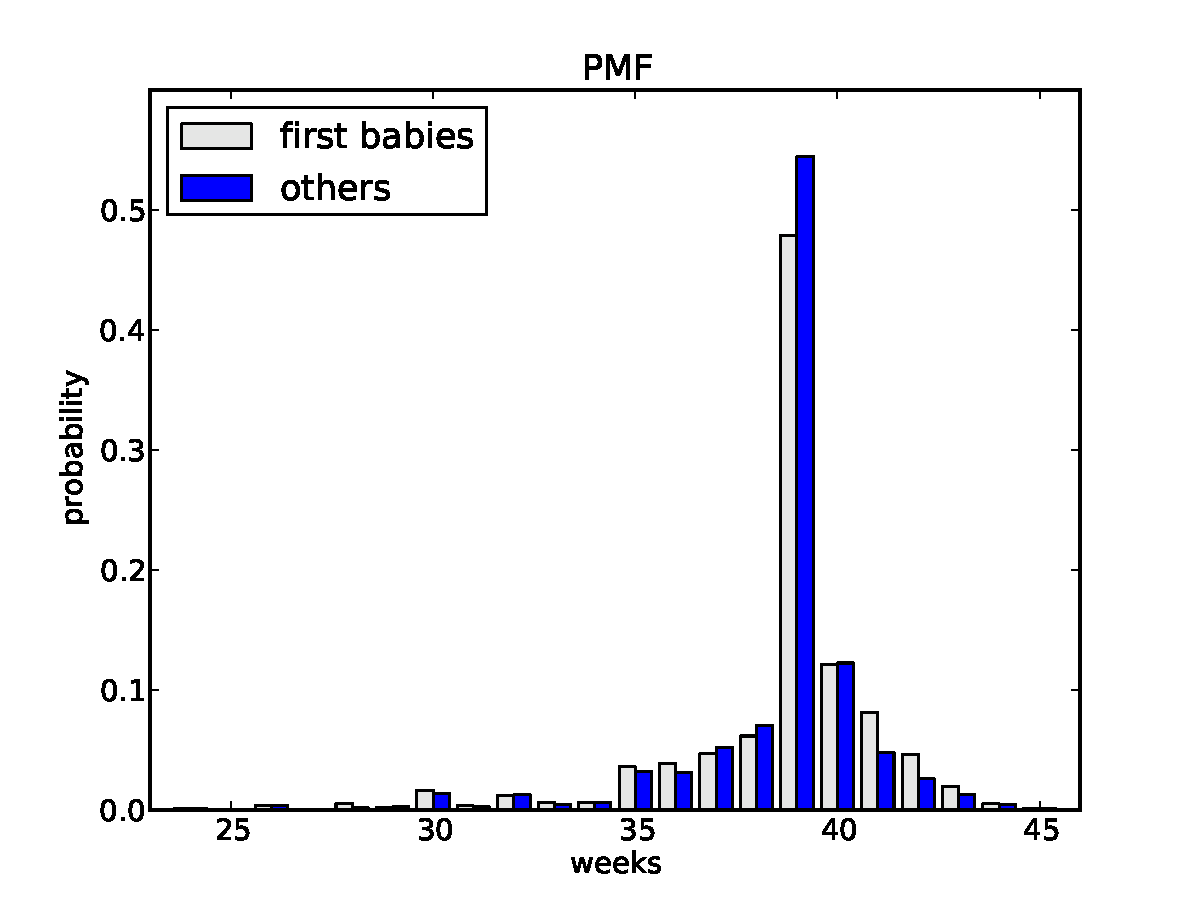
\includegraphics[height=2.5in]{figs/nsfg_pmf.pdf}}
\caption{PMF of pregnancy lengths.}
\label{nsfg_pmf}
\end{figure}
\index{pregnancy length}
\index{length!pregnancy}

Figure~\ref{nsfg_pmf} shows the PMF of pregnancy lengths as a bar
graph.  Using the PMF, we can see more clearly where the distributions
differ.  First babies seem to be less likely to arrive on time (week
39) and more likely to be a late (weeks 41 and 42).

The code that generates the figures in this chapters is available from
\url{http://thinkstats.com/descriptive.py}.  To run it, you will need the
modules it imports and the data from the NSFG (see
Section~\ref{nsfg}).
\index{National Survey of Family Growth}
\index{NSFG}
\index{{\tt descriptive.py}}

Note: {\tt pyplot} provides a function called {\tt hist} that
takes a sequence of values, computes the histogram and plots it.
Since I use {\tt Hist} objects, I usually don't use {\tt pyplot.hist}.


\section{Outliers}
\index{outlier}

Outliers are values that are far from the central tendency.  Outliers
might be caused by errors in collecting or processing the data, or
they might be correct but unusual measurements.  It is always a good
idea to check for outliers, and sometimes it is useful and appropriate
to discard them.

%weeks  count
%0      1
%4      1
%9      1
%13     1
%17     2
%18     1
%19     1
%20     1
%21     2
%22     7

In the list of pregnancy lengths for live births, the 10 lowest values
are \{0, 4, 9, 13, 17, 17, 18, 19, 20, 21\}.  Values below 20
weeks are certainly errors, and values higher than 30 weeks are
probably legitimate.  But values in between are
hard to interpret.
\index{pregnancy length}
\index{length!pregnancy}

On the other end, the highest values are:
%
\begin{verbatim}
weeks  count
43     148
44     46
45     10
46     1
47     1
48     7
50     2
\end{verbatim}

Again, some values are almost certainly errors,
but it is hard to know for sure.  One option is to {\bf trim} the data
by discarding some fraction of the highest and lowest values (see
\url{http://wikipedia.org/wiki/Truncated_mean}).
\index{trimmed mean}
\index{mean!trimmed}
\index{truncated mean}
\index{mean!truncated}


\section{Other visualizations}
\index{visualization}
\index{exploratory data analysis}

Histograms and PMFs are useful for exploratory data analysis;
once you have an idea what is going on, it is often useful to
design a visualization that focuses on the apparent effect.
\index{apparent effect}

In the NSFG data, the biggest differences in the distributions are
near the mode.  So it makes sense to zoom in on that part of the
graph, and to transform the data to emphasize differences.
\index{National Survey of Family Growth}
\index{NSFG}

Figure~\ref{nsfg_diffs} shows the difference between the PMFs for weeks
35--45.  I multiplied by 100 to express the differences in percentage
points.

\begin{figure}[ht]
% descriptive.py
\centerline{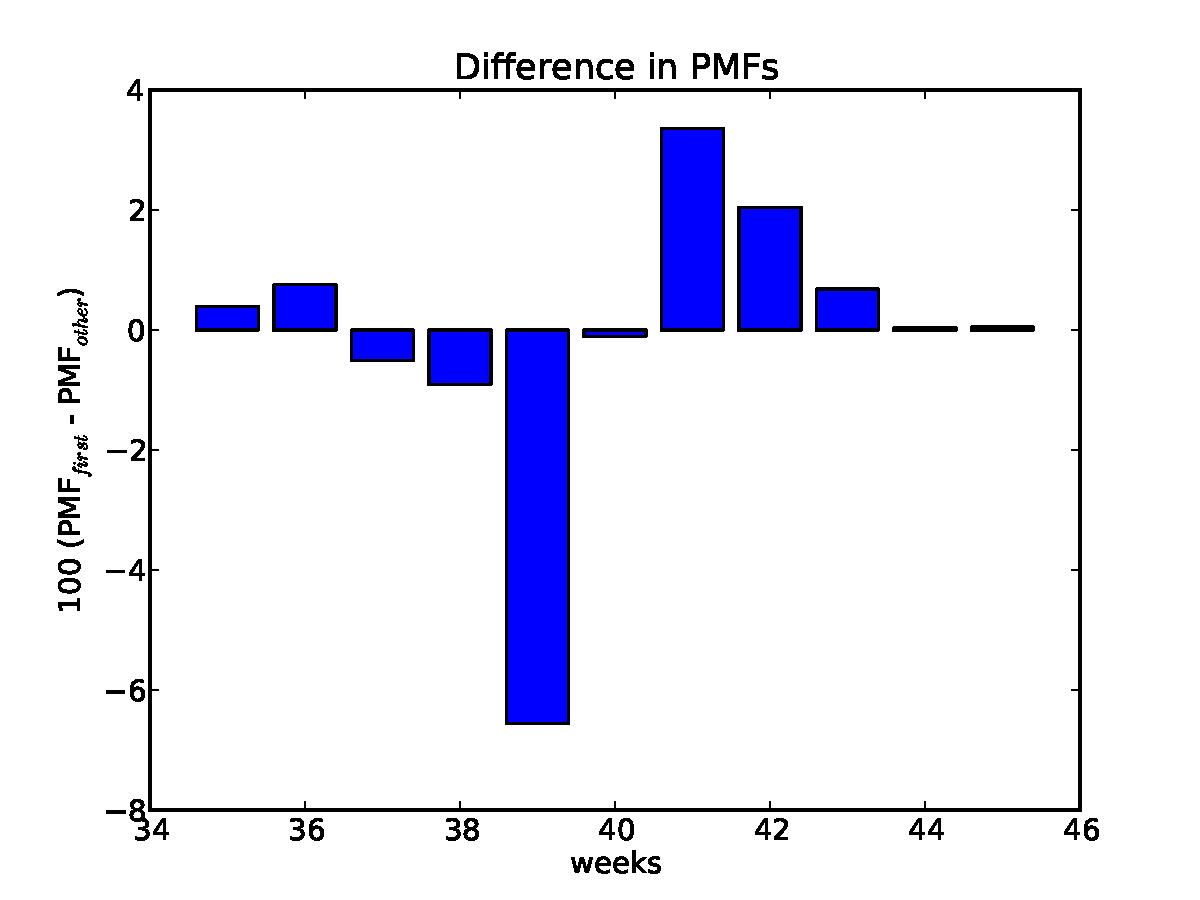
\includegraphics[height=2.5in]{figs/nsfg_diffs.pdf}}
\caption{Difference in percentage, by week.}
\label{nsfg_diffs}
\end{figure}

This figure makes the pattern clearer: first babies are
less likely to be born in week 39, and somewhat more likely
to be born in weeks 41 and 42.


\section{Relative risk}
\label{relative.risk}
\index{relative risk}

We started with the question, ``Do first babies arrive late?''  To
make that more precise, let's say that a baby is early if it is born
during Week 37 or earlier, on time if it is born during Week 38, 39 or
40, and late if it is born during Week 41 or later.  Ranges like these
that are used to group data are called {\bf bins}.
\index{bin}
\index{{\tt risk.py}}

\begin{exercise}
Create a file named {\tt risk.py}.
Write functions named {\tt ProbEarly}, {\tt ProbOnTime} and
{\tt ProbLate} that take a PMF and compute the fraction of births
that fall into each bin.  Hint: write a generalized function
that these functions call.

Make three PMFs, one for first babies, one for others, and one for
all live births.  For each PMF, compute the probability of being
born early, on time, or late.

One way to summarize data like this is with {\bf relative risk},
which is a ratio of two probabilities.  For example, the probability
that a first baby is born early is 18.2\%.  For other babies it is
16.8\%, so the relative risk is 1.08.  That means that first babies
are about 8\% more likely to be early.

Write code to confirm that result, then compute the relative risks of
being born on time and being late.  You can download a solution
from \url{http://thinkstats.com/risk.py}.

\end{exercise}


\section{Conditional probability}
\index{conditional probability}
\index{probability!conditional}

Imagine that someone you know is pregnant, and it is the beginning of
Week 39.  What is the chance that the baby will be born in the next
week?  How much does the answer change if it's a first baby?

We can answer these questions by computing a {\bf conditional
probability}, which is (ahem!) a probability that depends on a condition.
In this case, the condition is that we know the baby didn't arrive
during Weeks 0--38.

Here's one way to do it:

\begin{enumerate}

\item Given a PMF, generate a fake cohort of 1000 pregnancies.
For each number of weeks, $x$, the number of pregnancies with
duration $x$ is $1000 PMF(x)$.
\index{cohort}

\item Remove from the cohort all pregnancies with length less than 39.
\index{pregnancy length}
\index{length!pregnancy}

\item Compute the PMF of the remaining durations; the result is the
conditional PMF.

\item Evaluate the conditional PMF at $x = 39$ weeks.

\end{enumerate}

This algorithm is conceptually clear, but not very efficient.
A simple alternative is to remove from the distribution the values
less than 39 and then renormalize.

\begin{exercise}
Write a function that implements either of these algorithms and
computes the probability that a baby will be born during Week 39,
given that it was not born prior to Week 39.

Generalize the function to compute the
probability that a baby will be born during Week $x$, given that
it was not born prior to Week $x$, for all $x$.
Plot this value as a function of $x$ for first babies and others.

You can download a solution to this problem from
\url{http://thinkstats.com/conditional.py}.
\index{{\tt conditional.py}}

\end{exercise}


\section{Reporting results}

At this point we have explored the data and seen several apparent
effects.  For now, let's assume that these effects are real (but let's
remember that it's an assumption).  How should we report these
results?

The answer might depend on who is asking the question.  For example, a
scientist might be interested in any (real) effect, no matter how
small.  A doctor might only care about effects that are {\bf
  clinically significant}; that is, differences that affect treatment
decisions.  A pregnant woman might be interested in results that are
relevant to her, like the conditional probabilities in the previous
section.
\index{clinically significant}
\index{significance}

How you report results also depends on your goals.  If you are
trying to demonstrate the significance of an effect, you might choose
summary statistics, like relative risk, that emphasize differences.
If you are trying to reassure a patient, you might choose statistics
that put the differences in context.

\begin{exercise}
Based on the results from the previous exercises, suppose you were
asked to summarize what you learned about whether first
babies arrive late.

Which summary statistics would you use if you wanted to get a story
on the evening news?  Which ones would you use if you wanted to
reassure an anxious patient?
\index{Adams, Cecil}
\index{Straight Dope, The}

Finally, imagine that you are Cecil Adams, author of {\it The Straight
  Dope} (\url{http://straightdope.com}), and your job is to answer the
question, ``Do first babies arrive late?''  Write a paragraph that
uses the results in this chapter to answer the question clearly,
precisely, and accurately.

Forward~\ref{ex:rotate}.

\end{exercise}



\section{Glossary}

\begin{description}

\item[central tendency:] A characteristic of a sample or population;
intuitively, it is the most average value. 
\index{central tendency}

\item[spread:] A characteristic of a sample or population;
intuitively, it describes how much variability there is.
\index{spread}

\item[variance:] A summary statistic often used to quantify spread.
\index{variance}

\item[standard deviation:] The square root of variance, also used
as a measure of spread.
\index{standard deviation}

\item[frequency:] The number of times a value appears in a sample.
\index{frequency}

\item[histogram:] A mapping from values to frequencies, or a graph
that shows this mapping.
\index{histogram}

\item[probability:] A frequency expressed as a fraction of the sample
size.
\index{probability}

\item[normalization:] The process of dividing a frequency by a sample
size to get a probability.
\index{normalization}

\item[distribution:] A summary of the values that appear in a sample
and the frequency, or probability, of each.
\index{distribution}

\item[PMF:] Probability mass function: a representation of a distribution
as a function that maps from values to probabilities.
\index{PMF}

\item[mode:] The most frequent value in a sample.
\index{mode}

\item[outlier:] A value far from the central tendency.
\index{outlier}

\item[trim:] To remove outliers from a dataset.
\index{trim}

\item[bin:] A range used to group nearby values.
\index{bin}

\item[relative risk:] A ratio of two probabilities, often used to measure
a difference between distributions.
\index{relative risk}

\item[conditional probability:] A probability computed under the assumption
that some condition holds.
\index{conditional probability}

\item[clinically significant:] A result, like a difference between groups,
that is relevant in practice.
\index{clinically significant}

\end{description}


\begin{exercise}
Draw a stack diagram for \verb"print_n" called with
\verb"s = 'Hello'" and {\tt n=2}.
\end{exercise}

\begin{exercise}
Write a function called \verb"do_n" that takes a function
object and a number, {\tt n}, as arguments, and that calls
the given function {\tt n} times.
\end{exercise}

\begin{exercise}
\index{triangle}

If you are given three sticks, you may or may not be able to arrange
them in a triangle.  For example, if one of the sticks is 12 inches
long and the other two are one inch long, it is clear that you will
not be able to get the short sticks to meet in the middle.  For any
three lengths, there is a simple test to see if it is possible to form
a triangle:

\begin{quotation}
If any of the three lengths is greater than the sum of the other
  two, then you cannot form a triangle.  Otherwise, you
  can.  (If the sum of two lengths equals the third, they form
    what is called a ``degenerate'' triangle.)
\end{quotation}

\begin{enumerate}

\item Write a function named \verb"is_triangle" that takes three
  integers as arguments, and that prints either ``Yes'' or ``No,'' depending
  on whether you can or cannot form a triangle from sticks with the
  given lengths.

\item Write a function that prompts the user to input three stick
  lengths, converts them to integers, and uses \verb"is_triangle" to
  check whether sticks with the given lengths can form a triangle.

\end{enumerate}

\end{exercise}

\begin{exercise}
\label{ex:rotate}

ROT13 is a weak form of encryption that involves ``rotating'' each
letter in a word by 13 places.  To rotate a letter means
to shift it through the alphabet, wrapping around to the beginning if
necessary, so 'A' shifted by 3 is 'D' and 'Z' shifted by 1 is 'A'.
\index{letter rotation}
\index{rotation, letter}

Write a function called \verb"rotate_word"
that takes a string and an integer as parameters, and that returns
a new string that contains the letters from the original string
``rotated'' by the given amount.  

For example, ``cheer'' rotated by 7 is ``jolly'' and ``melon'' rotated
by -10 is ``cubed''.  

You might want to use the built-in functions {\tt ord}, which converts
a character to a numeric code, and {\tt chr}, which converts numeric
codes to characters.

Potentially offensive jokes on the Internet are sometimes encoded
in ROT13.  If you are not easily offended, find and decode some
of them.  Solution: \url{http://thinkpython.com/code/rotate.py}.
\end{exercise}

Backward~\ref{ex:rotate}.


We begin with a series of chapters on
graphical techniques, starting in Chapter \ref{ch:univariate} with
simple data sets consisting of only a single variable (or considering
only a single variable at a time), then moving on in Chapter

\label{ch:univariate}

\printindex

\clearemptydoublepage
%\blankpage
%\blankpage
%\blankpage


\end{document}

